\chapter{Constraints on Neutrino Lifetime}
\label{ch:lifetime}


The initial proposal to use solar neutrinos as a handle on neutrino lifetime explored a few models of neutrino decay and estimated that solar neutrinos could put the best limit on non-radiative neutrino decay~\cite{beacombell}.
The authors noted that the large uncertainty on the $^8B$ flux as well as uncertainties in the neutrino mass and mixing parameters would be a limiting factor.
Relatively recent precise mixing parameters from KamLAND~\cite{kamland} and Daya Bay~\cite{dayabay} and improved theoretical predictions for the $^8B$ flux~\cite{serenelli} mitigate this to some extent.
Further studies~\cite{berryman} using a simple disappearance model - where the neutrino decays into some non-active daughter(s) and the observable signal is an energy dependent distortion to the survival probability - were able to set respectable limits analyzing SNO~\cite{sno}, Super-Kamiokande~\cite{superk}, and Borexino~\cite{borexino} results.
Various constraints such as the eccentricity of the Earth's orbit allowed this limit to be improved~\cite{picoreti}. 
However, it was noted~\cite{berryman} that the published fits to the SNO data were not ideal for testing the simple disappearance model because the survival probabilities for electron neutrinos $P_{ee}$ and $P_{ea}$ were not treated as independent functions.
In a decaying scenario the survival probabilities are modified by an energy dependent form that does not preserve $P_{ee} + P_{ea} = 1$, so the authors concluded a better limit could be set with a dedicated fit.
This analysis aims to perform such a dedicated fit, specifically for the neutrino mass state 2 lifetime observed as an energy dependent modification to the standard Mikheyev - Smirnov - Wolfenstein (MSW)~\cite{wolfenstein,mikheyev} survival probability.

\section{Lifetime Model}
\label{lifetime_model}

To fit for neutrino lifetime using SNO data one first needs a model of the survival probability curves.
The fit will minimize the negative SNO Enhanced Log Likelihood function~\cite{plthesis} using this model for the survival probability.
The following sections discuss the model itself and the treatment of parameters.

\subsection{Decaying Survival Probability}

The flux of a particular mass state $\ket{\nu_i}$ could have some lifetime associated with it $\tau_i$ representing the decay of neutrinos of that mass state.
Since the actual neutrino masses are unknown the lifetime is often represented by an effective parameter $k_i$ scaled by the mass of the state
\begin{equation}
k_i = \frac{\tau_i}{m_i}.
\end{equation}
Since the Earth-Sun distance is so large compared to the solar radius any decay within the sun will be ignored. 
Therefore, using the formalism given in \Cref{ch:theory}, the detected flux $\psi_i$ of a neutrino mass state at earth can be given as 
\begin{equation}
\psi_i \approx  e^{-L_\odot / (E k_i)} \phi_i =  e^{-L_\odot / (E k_i)} \left| \braket{\nu_{m i}(V_e)}{\nu_e} \right|^2
\label{decay}
\end{equation}
The standard survival probabilities for electron and muon/tau flavor neutrinos may then be recovered with appropriate factors from the PMNS matrix and fed into QSigEx (the 3-phase fitter developed by Pierre-Luc Drouin~\cite{plthesis}).
\begin{equation}
\begin{array}{rcl}
P_{ee} & = & \sum_i \psi_i |U_{ie}|^2  \\
P_{ea} & = & \sum_i \psi_i |U_{i\mu}|^2 + \psi_i |U_{i\tau}|^2
\end{array}
\label{survive}
\end{equation}

\subsection{Monte-Carlo Simulation}

\label{montecarlo}

Since $^8$B solar neutrinos are produced in a continuous region of the sun which samples a range of electron densities, a model seeking to fit a shape change should well reproduce this effect.
See \Cref{fig:core_density} for a visual representation of the magnitude of this effect.

\begin{figure}
\centering
\includegraphics[width=0.75\columnwidth]{survival_core}
\caption{The solid lines here represent the MSW survival probability curves for neutrinos at the center of the solar core, with neutrinos produced a $0.1R_{\odot}$ in dashed lines. Most $^8$B neutrinos come from intermediate densities.}
\label{fig:core_density}
\end{figure}

To calculate the survival probability for a particular neutrino energy value, a Monte-Carlo simulation generates initial electron neutrino states for $^8$B decays at radial positions sampled from the SSM distribution for $^8$B neutrino flux.
The SSM electron density distribution is then used to convert the radial position inside the Sun to an electron density.
To get the matter mass state composition the the Hamiltonian $H_{MSW}$ is first converted to the flavor basis with the PMNS matrix and then the eigenvectors are calculated numerically using TMatrixDEigen from ROOT 6.5.34~\cite{root}.
These eigenvectors are $\ket{\nu_{mi}(V_e)}$, and their projection onto $\ket{\nu_e}$, which is trivial in the flavor basis, yields \Cref{rawflux}.

The final flux of a mass state without decay is calculated from the average of all the neutrino states.
These fluxes are then decayed according to \Cref{decay} for a particular lifetime value and the survival probabilities from \Cref{survive} are used to check the goodness of fit to the data.
Example survival probability curves for different lifetime values are shown in \Cref{fig:model}.

\begin{figure}
\centering
\includegraphics[width=0.75\columnwidth]{decay_msw_theory}
\caption{
The electron neutrino survival probability curves from the Monte-Carlo simulation that underlies this analysis for various values of the lifetime. The shaded regions represent the propagated error from the neutrino mixing parameter priors while the solid lines are the central values.
}
\label{fig:model}
\end{figure}

\subsection{Parameters}
\label{parameters}

The lifetime model and monte-carlo simulation require the parameters discussed in the following sections to produce the survival probability curves.
Nuisance parameters in the analysis are treated exactly as described in~\cite{plthesis}.
Fundamental constants are taken from the PDG~\cite{pdg}.

\subsubsection{Neutrino Lifetime}
The three neutrino mass states each have a lifetime associated with them $k_i = \tau_i / m_i$. 
For this analysis the lifetimes of mass state 1 and 3 are fixed at infinity because the $^8B$ flux exits the sun as a nearly pure $\nu_2$ mass state, so the data taken by SNO for $^8$B neutrinos is nominally insensitive to $\nu_1$ or $\nu_3$ decay.
This is shown in \Cref{fig:frac_not_nu_2} which uses the central values from the following section to compute the fraction of $^8$B neutrinos exiting the sun that are not $\nu_2$.

\begin{figure}
\centering
\includegraphics[width=0.75\columnwidth]{fraction_not_nu_2}
\caption{
The fraction of $^8$B neutrinos that are not mass state $\nu_2$ upon exiting the sun are shown here as a function of neutrino energy. This plot was created using the central values for the neutrino and solar parameters. 
}
\label{fig:frac_not_nu_2}
\end{figure}

\subsubsection{Neutrino Mixing}
Neutrino mixing parameters taken from KamLAND~\cite{kamland} and DayaBay~\cite{dayabay} are reproduced in \Cref{tbl:mixing_params}. 
Parameters from KamLAND and DayaBay were used to avoid bias from using SNO results in this analysis.
As these measurements were done at Earth with neutrinos produced on Earth they are expected to be uncorrelated with effects of $\nu_2$ decay.
The current limit on $k_2$ constrains it to be greater than $\approx7\times10^{-4}$~\cite{picoreti} which means at length scales comparable to the diameter of the earth the maximum flux lost by $\nu_2$ decay for a $10$ MeV neutrino is given by
$1-e^{-2R_{earth}/(E k_2)} \approx 6\times10^{-6}$
which would have negligible impact on values quoted for mixing parameters.
These parameters and their central values are used as priors and floated during the fit.
See \Cref{systematics} for further discussion.

\begin{table}
\centering
\begin{tabular}{c|c|c}
Parameter & Value & Ref \\ \hline
$ \Delta m ^2 _{21} $ & $7.58^{+0.14}_{-0.13}(stat)^{+0.15}_{-0.15}(syst) \times 10^{-5}$ eV$^2$ & \cite{kamland} \\ \hline
$ \tan^2 \theta_{12} $ & $0.56^{+0.10}_{-0.07}(stat)^{+0.10}_{-0.06}(syst) $ & \cite{kamland} \\ \hline
$ |\Delta m ^2 _{32}| $ & $2.45\pm0.06(stat)\pm0.06(syst) \times 10^{-3}$ ev$^2$ & \cite{dayabay} \\ \hline
$ \sin^2 2\theta_{13} $ & $0.0841\pm0.0072(stat)\pm0.0019(syst)$ & \cite{dayabay} \\ \hline
$ \sin^2 \theta_{23} $ & $0.5^{+0.058}_{-0.062}$ & \cite{superkth23} \\ 
\end{tabular}
\caption{
\label{tbl:mixing_params}
Reproduced here are the mixing parameters used in this analysis taken from Daya Bay~\cite{dayabay}, Super Kamiokande~\cite{superkth23}, and KamLAND~\cite{kamland} results.
}
\end{table}

\subsubsection{Standard Solar Model}

The model implemented here uses the distribution of electron density and distribution of neutrino fluxes calculated in the BS05(OP) Standard Solar Model (SSM)~\cite{bs05op} which are reproduced in \Cref{fig:ssm}. 
Uncertainties in these values are not quoted in the original source and are therefore not considered in this fit.
These predictions are expected to be uncorrelated with $\nu_2$ decay as they are not constrained with neutrino flux measurements.

\begin{figure}
\centering
\includegraphics[width=0.48\columnwidth]{ssm_ne}
\includegraphics[width=0.48\columnwidth]{ssm_nu_region}
\caption{
The electron density in the Sun as a function of radius and the fraction of the neutrino flux produced in a radial region as a function of radius for the different neutrino fluxes. Only the $^8$B flux is relevant for this data. From the BS05(OP) SSM~\cite{bs05op}.
}
\label{fig:ssm}
\end{figure}

\subsubsection{$^8$B Flux}

As earth bound measurements of the solar neutrino flux would be biased by neutrino decay, a theoretical prediction for the $^8$B flux is required.
Serenelli's most recent prediction yields a $^8$B flux of $5.88\times10^{6}$ cm$^-2$s$^-1$ with $11\%$ uncertainty~\cite{serenelli} which is used as a prior in this fit.
For reference the flux from BS05(OP)~\cite{bs05op} is $5.69\times10^6$ cm$^-2$s$^-1$.
See \Cref{strategy} for further discussion of how the flux is treated in the fit.

\section{Fit Implementation}
\label{fit_impl}

Since this analysis is (only) proposing a survival probability model to be considered when fitting SNO data, and many analyses have already been written and vetted for fitting survival probability models, it was decided to build off an existing and vetted fit that properly handled nuisance parameters, pdf generation, data binning, and likelihood function implementation.

\subsection{QSigEx}

Three phase fits to SNO data that treated $P_{ee}$ and $P_{ea}$ independent polynomials existed in the software package QSigEx~\cite{plthesis}.
This package already implemented the SNO Enhanced Log Likelihood Function, and it was relatively easy to modify the fits to use the model described in \Cref{lifetime_model} instead of polynomials.
Since QSigEx was previously vetted for SNO fits, a demonstration that the updated code produces the same results as previous analyses is given in \Cref{qsigex_validation}.
For this analysis, then, the focus is on demonstrating that the fit in the updated code is an unbiased estimator of the neutrino lifetime of mass state two, given the assumptions discussed previously. 

\subsection{Signal Extraction}

This by and large follows the scheme layed out in Section 5 of Pierre-Luc's thesis~\cite{plthesis} where it is described in exquisite detail. 
The deviation here occurs only in that instead of polynomial parameters, the parameters in discussed in \Cref{parameters} are used in the fit.

\subsection{Neutrino Energy Binning}

Pierre-Luc discussed two varieties of fit in his thesis.
\begin{itemize}
\item Binned neutrino energy fits where where the neutrino monte-carlo is binned into $N$ PDFs by neutrino energy prior to the fit, and the average value of the survival probability across that entire bin is applied to each of the $N$ PDFs when stepping though the minimization.
\item Unbinned neutrino energy fits where each of the $M >> N$ neutrino monte-carlo events are reweighted by the value of the survival probability at their exact energy when stepping through the minimization to build the neutrino PDFs.
\end{itemize}
Clearly the binned fit will perform more poorly as an average value of the survival probability across a neutrino energy bin is applied to all neutrinos in that bin, however this method is much faster being computationally far simpler than rebuilding the PDFs at each minimization step. 
For polynomial fits this poorer performance was not significant and allowed the systematic scans along with the shifts and refits to benefit from the speed increase.
Unfortunately as discussed in \Cref{polynomial_tests} the binned fit performed very poorly at capturing the shape of the lifetime model survival probabilities.
Because of this, only the unbinned neutrino energy fit is considered in the following sections.

\section{Fit Strategy}
\label{strategy}
Ideally all neutrino parameters would be floated with priors in this fit. 
In practice it has been observed that the fit does not converge with both the $^8$B flux and lifetime parameter floated unless there is a very strong external constraint on the flux (see \Cref{lifetime_and_flux}).
Previous analyses \cite{plthesis} have encountered a similar issues and opted for a strategy of finding a preferred $^8$B flux in some reduced fit and then performing further fits and statistical studies with the flux fixed.
In this analysis since there is only one model parameter of interest, $k_2$, a strategy of scanning $k_2$ manually while floating all other parameters seems to be ideal. 
With that in mind, the current strategy is:
\begin{enumerate}
\item Perform a scan over $k_2$ minimizing floated parameters at each point. For data fits this can be done along with the other scanned nusiance parameters. (See Section 5.4.2 in \cite{plthesis})
\item At the best $\chi^2$ value, use MINOS fit errors (implicitly with $k_2$ fixed) as the total uncertainty on all parameters except the highly correlated $k_2$ and $^8$B flux.
\item For $k_2$ find the total uncertainty by at the point where $\Delta(-LL)$ in the scan is $0.5$.
\item For the total uncertainty on $^8$B flux this value is scanned the same way as $k_2$ to properly account for the correlations in with $k_2$.
\item Combine with these uncertainties on $k_2$ and the $^8$B flux additional shift and refit uncertainties from scanned nuisance parameters.
\end{enumerate}

\section{Ensemble Testing}
\label{ensemble_tests}

The purpose here is to demonstrate that the fit is unbiased and correctly estimating errors on the fitted parameters. 
These tests were heavily inspired by Section 6 of Pierre-Luc's thesis~\cite{plthesis}.
Figures of merit shown here include the pull, the bias, and the relative uncertainty.
\begin{equation}
Pull = \frac{Fit\,\,\,value - Actual\,\,\,value}{Fit\,\,\,uncertainty}
\end{equation}
\begin{equation}
Bias = \frac{Fit\,\,\,value - Actual\,\,\,value}{Actual\,\,\,value}
\end{equation}
\begin{equation}
Relative\,\,\,uncertainty = \frac{Fit\,\,\,uncertainty}{Actual\,\,\,value} \times 100\%
\end{equation}
For the bias and pull, the mean of each ensemble is shown with error bars representing the standard deviation of the ensemble.
The pull plots will additionally show the expected fluctuation of the mean ($1/\sqrt{n_{samples}}$) in dashed lines with the expected mean ($1 - 1/(4(n_{samples}-1))$) and fluctuation of the standard deviation ($1/\sqrt{n_{samples}}$) represented by shaded boxes.
For relative uncertainty only the mean of the ensembles is shown.

\subsection{Fake Datasets}

The SNO MC consists of different event classes for each phase of SNO.
Events from each class and phase are partitioned into $N$ sets with $M$ samples each. 
The remaining unused MC data for each phase and class is used for PDFs in the fit, so $N$ must be chosen to leave sufficient uncorrelated data for PDF generation.
$M$ is chosen from a Poisson distribution with a mean equal to the expected number of events for that event class and phase from previous SNO analyses~\cite{leta,ncd,3phase}.
For solar neutrino signals the BS05(OP)~\cite{bs05op} flux predictions were used in generating these fake data sets.
The full list of Poisson means $M$ and the number of generated sets $N$ are given in Appendix C of Pierre-Luc's thesis~\cite{plthesis}.
These sets can then be combined into fake datasets with realistic statistics containing only the event classes and phases desired.

%\begin{figure}
%\centering
%\begin{tabular}{l||c|c|c|c}
%Phase/Class & Total Events & Poisson Mean & Gen'd Sets & Remaining \\ \hline
%& & & & \\ \hline 
%& & & & \\ 
%\end{tabular}
%\caption{
%The poisson means used in generating fake data sets along with the total number of generated sets for each signal class and phase.
%Additionally shows the total number of events generated in SNO MC and the number of uncorrelated events remaining for PDFs in the fits.
%}
%\label{tbl:fake_means}
%\end{figure}

The solar neutrino signals from SNO monte-carlo, which were generated with a flat survival probability spectrum, were reweighted with the lifetime model as described in \ref{lifetime_model}. 
A representative value of $k_2 = 10^{-4}$ s/eV was seeded into the fake sets to test the fit performance near the current limit of $\approx7\times10^{-4}$~\cite{picoreti}.

\subsection{Solar-Signal Only}
\label{3phase_sigonly}

\begin{table}
\centering
\begin{tabular}{ccc}
\hline
D$_2$0 Phase Event Classes & Salt Phase Event Classes & NCD Phase Event Classes  \\ \hline \hline
$^8$B CC & $^8$B CC & $^8$B CC \\
$^8$B ES (e) & $^8$B ES (e) & $^8$B ES (e) \\
$^8$B ES ($\mu\tau$) & $^8$B ES ($\mu\tau$) & $^8$B ES ($\mu\tau$) \\
$^8$B NC & $^8$B NC & $^8$B NC \\ \hline
\end{tabular}
\caption{
The solar-signal event classes included from LETA and NCD(-PMT) phases. Note that NCD-NCD data was not included explicitly in the fit but comes into play as the PSA constraint~\cite{3phase}.
}
\label{tbl:sigonly_evcls}
\end{table}

It was possible to create 250 uncorrelated datasets of solar-signal only data.
The solar-signal event classes for LETA and NCD phases are shown in \Cref{tbl:sigonly_evcls}.
With QSigEx configured to only fit these event classes, the lifetime fit was performed on each dataset as described in \Cref{strategy}. 
The figures of merit for these tests are shown in \Cref{fig:sigonly_biaspull,fig:sigonly_reluncert}. 
In short, the results are consistent with an unbiased fit that properly estimates the fit uncertainties.

\begin{figure}
\centering
\includegraphics[width=0.85\columnwidth]{bias_nofit}
\includegraphics[width=0.85\columnwidth]{pull_nofit}
\caption{
The bias and pull of all fitted parameters with signal only datasets. Gray bars and dashed lines represent expected fluctuations due to limited statistics.
}
\label{fig:sigonly_biaspull}
\end{figure}

\begin{figure}
\centering
\includegraphics[width=0.85\columnwidth]{reluncert_nofit}
\caption{
The relative uncertainty of all fitted parameters with signal only datasets.
}
\label{fig:sigonly_reluncert}
\end{figure}

\subsection{Solar-Signal + High Statistics Backgrounds}

\begin{table}
\centering
\begin{tabular}{ccc}
\hline
D$_2$O Phase Backgrounds & Salt Phase Backgrounds & NCD Phase Backgrounds \\ \hline \hline
AV neutrons & AV neutrons & External neutrons \\
Bi D$_2$O & Bi Salt & D$_2$O p.d. \\ 
Tl D$_2$O & Tl Salt & Atmospherics \\
hep CC & hep CC & hep CC \\
hep ES & hep ES & hep ES \\
hep NC & hep NC & hep NC \\
PMT $\beta$-$\gamma$ & PMT $\beta$-$\gamma$ \\ \hline
\end{tabular}
\caption{
These are the background event classes that are included in the high statistics background tests. Note that NCD-NCD data is not in the fit but is included with the PSA constraint. This includes internal backgrounds, AV neutrons, PMT backgrounds, and other backgrounds with very high Monte-Carlo statistics.
}
\label{tbl:noextbitl_event_classes}
\end{table}

A subset of the fake 3-phase solar-signal only datasets from both LETA phases and NCD phase above were taken and combined with uncorrelated datasets of background events with high statistics.
The event classes shown in \Cref{tbl:noextbitl_event_classes} were added in this section. 
Due to the relatively lower statistics for background event classes, only 50 datasets could be created for each of the three $k_2$ values.
With QSigEx configured to only fit these event classes, the lifetime fit was performed on each dataset as described in \Cref{strategy}. 
The figures of merit for these tests are shown in \Cref{fig:noextbitl_bias,fig:noextbitl_pull,fig:noextbitl_reluncert}. 
Again, the results are consistent with an unbiased fit that properly estimates the fit uncertainties.

\begin{figure}
\centering
\includegraphics[width=0.85\columnwidth]{noextbitl_bias_nofit}
\caption{
The bias of all fitted parameters with signal + high stats backgrounds datasets.
}
\label{fig:noextbitl_bias}
\end{figure}

\begin{figure}
\centering
\includegraphics[width=0.85\columnwidth]{noextbitl_pull_nofit}
\caption{
The pull of all fitted parameters with signal + high stats backgrounds datasets. Gray bars and dashed lines represent expected fluctuations due to limited statistics.
}
\label{fig:noextbitl_pull}
\end{figure}

\begin{figure}
\centering
\includegraphics[width=0.85\columnwidth]{noextbitl_reluncert_nofit}
\caption{
The relative uncertainty of all fitted parameters with signal + high stats backgrounds datasets.
}
\label{fig:noextbitl_reluncert}
\end{figure}

\subsection{Solar-Signal + All Backgrounds}
\label{3phase_allbg}

\begin{table}
\centering
\begin{tabular}{ccc}
\hline
D$_2$O Phase Backgrounds & Salt Phase Backgrounds & NCD Phase Backgrounds\\ \hline \hline
Bi AV bulk & Bi AV bulk & Strings p.d. \\
Tl AV bulk & Tl AV bulk & K2 p.d. \\
Bi H$_2$O & Bi H$_2$O & K5 p.d. \\
Tl H$_2$O & Tl H$_2$O & \\ \hline
\end{tabular}
\caption{
These are the background event classes that are added for the fits that include all backgrounds. Note that NCD-NCD data is not in the fit but is included with the PSA constraint. This includes AV and external backgrounds for LETA and photodisintegration for NCD phase.
}
\label{tbl:allbg_event_classes}
\end{table}

A subset of the fake 3-phase high statistics background datasets from above were taken and combined with uncorrelated datasets of background events classes with low statistics.
The event classes shown in \Cref{tbl:allbg_event_classes} were added in this section and the datasets now include all relevant event classes.
Due to extremely limited statistics for some of these event classes, only 14 datasets for each of the three $k_2$ values could be created.
As was traditionally done for SNO analyses~\cite{plthesis}, these same events were resampled with a different random seed into 14 alternate datasets (c.f. the bootstrap method).
Comparing the results of these two datasets gives some information on statistical fluctuations due to limited statistics.
If the bias or pull looks particularly bad in one dataset but acceptable in the other, one can conclude that this effect is due to statistical fluctuations and not to errors in the fit procedure.
The figures of merit for these tests are shown in \Cref{fig:allbg_bias,fig:allbg_pull,fig:allbg_reluncert}. 
While fluctuations are larger, comparison between the two datasets looks more reasonable. 
Notably these results are comparable to ensemble testing of the published SNO 3-phase results as shown in Pierre-Luc's thesis~\cite{plthesis}.
One can therefore conclude that the fit is unbiased and properly predicting errors.

\begin{figure}
\centering
\includegraphics[width=0.85\columnwidth]{bias_combined}
\caption{
The bias of all fitted parameters with signal + all backgrounds datasets. The alternate ensemble results are shown in green for comparison.
}
\label{fig:allbg_bias}
\end{figure}

\begin{figure}
\centering
\includegraphics[width=0.85\columnwidth]{pull_combined}
\caption{
The pull of all fitted parameters with signal + all backgrounds datasets. Gray bars and dashed lines represent expected fluctuations due to limited statistics. The alternate ensemble results are shown in green for comparison.
}
\label{fig:allbg_pull}
\end{figure}

\begin{figure}
\centering
\includegraphics[width=0.85\columnwidth]{reluncert_combined}
\caption{
The relative uncertainty of all fitted parameters with signal + all backgrounds datasets. The alternate ensemble results are shown in green for comparison.
}
\label{fig:allbg_reluncert}
\end{figure}

\clearpage 

\section{Detector Systematic Effects}
\label{systematics} 

Section 5.4 of Pierre-Luc's thesis~\cite{plthesis} covers the strategy used here in great detail. 
A summary of that strategy follows. A million sets of randomly sampled systematic parameters are produced by sampling asymmetric Gaussian distributions of parameter uncertainties. These distributions are either known from independent analyses or determined by initial scans of the dataset. For each set of parameters, the fit is minimized again and the most likely value of each parameter is recorded. The RMS of these shift-and-refit $k_2$ values on each side of the central value for $k_2$ are calculated as the systematic effect. Both positive and negative uncertainties are quoted but it is important to note that this analysis is expected to produce a lowerbound on $k_2$ making the positive error rather meaningless.

The following systematic tests were done at the best fit values for a fake dataset of comparable statistics to the SNO 3 phase dataset. This fake dataset was seeded with $k_2 = 10^{-4}$ and had the $^8$B flux seeded and fixed at the SSM central value.

The parameters considered here include nuisance parameters and all parameters scanned as the preliminary step in the fit. The scans are reproduced in \Cref{fake_scan} while \Cref{fig:detector_systematics1,fig:detector_systematics2} show the individual contributions of the scanned parameters to the detector systematic uncertainty on $k_2$: $^{+13.4\%}_{-9.03\%}$.

\begin{figure}
\centering
\includegraphics[width=0.95\columnwidth]{basic_1_2}
\caption{The calculated systematic effect on $k_2$ from the first half of the detector systematic parameters in the fit is shown here. Red represents positive (blue, negative) fractional error.}
\label{fig:detector_systematics1}
\end{figure}

\begin{figure}
\centering
\includegraphics[width=0.95\columnwidth]{basic_2_2}
\caption{The calculated systematic effect on $k_2$ from the second half of the detector systematic parameters in the fit is shown here. Red represents positive (blue, negative) fractional error.}
\label{fig:detector_systematics2}
\end{figure}


%\section{Injected Signal}
%
%The plan here is to inject a fake signal into real data by removing events from the $1/3$ dataset.
%To decide which events to remove, a fake (Monte-Carlo) dataset comprising of only the solar-signal event classes with a mean number of events for each event class set to correspond to the $1/3$ dataset will be reweighted into two distinct datasets: one with infinite lifetime and one with a finite and small lifetime ($10^{-4}$ s/eV). 
%These two datasets will be binned as in the actual fit producing a PDF for each lifetime condition for each signal of each phase.
%The PDFs for the finite and infinite lifetime cases will be summed across the solar-signal classes for each phase, producing a finite and infinite lifetime solar-signal PDF for each phase.
%The deficit of events in the finite lifetime PDF relative to the infinite lifetime PDF for a particular phase determines how many events should be removed from the $1/3$ dataset in the same bin to inject that signal into that dataset.
%The fit can then be run on the signal-injected $1/3$ dataset to check the bias and pull of the fit.
%This will demonstrate that the fit works on real data without actually fitting to a real signal in the data.

\clearpage

\section{\nicefrac{1}{3} Dataset}
\label{third}

Using 1/3 of the SNO dataset --- the same 1/3 dataset used in testing the historical 3-phase fits --- the fit was run as described in \Cref{strategy}. 
To reduce computational power required for this test, the central values of scanned nuisance parameters from Pierre-Luc's 3-phase Pee+Pea fit were used. 
These are nominally uncorrelated with neutrino parameters, and would take a very long time to iteratively scan with little gain.
This scan will, of course, be done for the full dataset.
The scan of $k_2$ and the $^8$B flux are shown in \Cref{fig:third_scans}.
The neutrino parameters are shown relative to their priors in \Cref{fig:priors_third}.
The observable projections for the minimum and with $k_2$ fixed to infinity are shown in \Cref{third_observables}.

There is a 1-sigma minimum for $k_2$ at a central value of of $4.62\times10^{-4}$ s/eV.
This minimum is almost consistent with infinite lifetime at the one sigma level, and has a one sigma lower bound of $2.40\times10^{-4}$ s/eV.
The fitted value of the $^8$B flux is $5.77^{+0.58}_{-0.58}\times10^6$ cm$^{-2}$s$^{-1}$ ($1.01\pm0.10 \times \Phi_{8B_{BS05(OP)}}$) which is quite consistent with the SSM predictions.
With $k_2$ fixed at infinity the $^8$B flux fits to $5.19^{+0.16}_{-0.16}\times10^6$ cm$^{-2}$s$^{-1}$ ($0.91\pm0.03 \times \Phi_{8B_{BS05(OP)}}$).
Both flux measurements are consistent with previous 3-phase SNO results: $5.23^{+0.16}_{-0.16}\times10^6$ cm$^{-2}$s$^{-1}$ ($0.92\pm0.03 \times \Phi_{8B_{BS05(OP)}}$).

\begin{figure}
\centering
\includegraphics[width=0.95\columnwidth]{k2_scan_third} \\
\vspace{12pt}
\includegraphics[width=0.95\columnwidth]{flux_scan_third}
\caption{The scans of $k_2$ and the $^8$B flux for the 1/3 dataset. The red points are the scan values, and the blue line is a fit to the minimum.}
\label{fig:third_scans}
\end{figure}

\begin{figure}
\centering
\includegraphics[width=0.95\columnwidth]{prior_deviation_third}
\caption{The fractional deviation of each neutrino parameter with a prior constraint from its prior. The errors shown are the fractional errors of the fit.}
\label{fig:priors_third}
\end{figure}

\clearpage

\section{Final Results}
\label{final}

Now with the entire SNO dataset, the fit was run as described in \Cref{strategy}. 
As a preliminary step, the systematics identified in the previous 3-phase analysis as requiring scanning were scanned iteratively until a global minimum was found.
An important caveat to point out is that a $\beta_{14}$ scale parameter became stuck on a non-physical discontinuity in the likelihood space for two iterations of the scan (the second and third).
By nonphysical I mean that the scanned range of this systematic was large enough to shift the $\beta_{14}$ cut applied when skimming the MC into the the $\beta_{14}$ ROI, ultimately resulting in a discontinuous jump in the likelihood.
Manually correcting this fit and limiting the scanned range of this parameter resulted in successful minimization and convergence for the remaining scans.
For clarity, the scans shown in \Cref{final_syst_scan_omit} omit the second and third scans, while for completeness, \Cref{final_syst_scan} shows all the scans. 
Using the central values for the systemtics shown in the scan, both $k_2$ and $^8$B flux were then scanned with the systematic parameters fixed at their central values, and are shown in \Cref{fig:final_scans}.
The neutrino parameters are shown relative to their priors at the minimum of this scan in \Cref{fig:priors_final}.
The observable projections for the minimum and with $k_2$ fixed to infinity are shown in \Cref{final_observables}.

To account for systematic effects, a shift-and-refit procedure was applied to stochastically marginalize over the systematic parameters.
$10^6$ sets of systematic parameters were drawn from asymmetric Gaussian distributions representing the uncertainty on each parameter. 
The fit was run with each set of shifted systematic parameters producing distributions of shifts in each floated parameter by comparing shifted fit results with the results from the central fit.
An assumption was made that the small shifts in any floated parameter does not change the shape of the likelihood profile for that parameter, but rather only shifts the most likely value. 
Taking this assumption, a final likelihood profile can be produced for $k_2$ by averaging the shifted likelihood profile obtained with systematics fixed at their central values by the distribution of $k_2$ shifts obtained in the shift-and-refit procedure.
This likelihood is compared to the likelihood profile without systematics in \Cref{fig:systematic_scans}.
The parameter $k_2$ was treated in this way due to highly asymmetric errors. 
For other parameters, an asymmetric Gaussian is fit to the distribution of fitted values from the shift-and-refit procedure and these upper and lower widths are added in quadrature with the upper and lower widths uncertainties from the central fit.

The minimum for $k_2$ observed in the 1/3 data fit is still present in this fit (at higher significance) at a central value of of $3.45^{+5.50}_{-1.68}\times10^{-4}$ s/eV where the uncertainty given is the total uncertainty
This minimum is consistent with infinite lifetime at a bit over $85\%$ confidence, and sets a $90\%$ confidence lower bound at $>8.08\times10^{-5}$ s/eV.
This lower bound was found by applying Wilks' theorem to the systematically broadened likelihood, i.e. when the $-2\Delta\log{L}$ from the minimum crosses $2.71$.
The fitted value of the $^8$B flux is $6.08^{+0.47}_{-0.47}$(stat.)$^{+0.21}_{-0.22}$(syst.)$\times10^6$ cm$^{-2}$s$^{-1}$ ($1.07\pm0.10 \times \Phi_{8B_{BS05(OP)}}$) which is quite consistent with the SSM predictions and constraint.
With $k_2$ fixed at infinity the $^8$B flux fits to $5.22^{+0.16}_{-0.16}\times10^6$ cm$^{-2}$s$^{-1}$ ($0.92\pm0.03 \times \Phi_{8B_{BS05(OP)}}$).
The flux measurement with $k_2$ fixed at infinity is expected to reproduce previous 3-phase results, and is quite consistent consistent with those results: $5.23^{+0.16}_{-0.16}\times10^6$ cm$^{-2}$s$^{-1}$ ($0.92\pm0.03 \times \Phi_{8B_{BS05(OP)}}$).
There is some tension between the SNO result and the flux fitted with with $k_2$ floating, however they are consistent at two sigma. 

\begin{figure}
\centering
\includegraphics[width=0.95\columnwidth]{k2_scan_final} \\
\vspace{12pt}
\includegraphics[width=0.95\columnwidth]{flux_scan_final}
\caption{The scans of $k_2$ and the $^8$B flux for the full dataset. The red points are the scan values, and the blue line is a fit to the minimum.}
\label{fig:final_scans}
\end{figure}

\begin{figure}
\centering
\includegraphics[width=0.95\columnwidth]{sno_8b_stat_syst_profile.pdf}
\caption{The scans of $k_2$ with and without systematic effects. Note that in both cases the minimum has been shifted to zero. With systematics included the minimum is less significant relative to the limiting value at $k_2 \rightarrow \infty$ as expected.}
\label{fig:systematic_scans}
\end{figure}

\begin{figure}
\centering
\includegraphics[width=0.95\columnwidth]{prior_deviation_final}
\caption{The fractional deviation of each neutrino parameter with a prior constraint from its prior. The errors shown are the fractional errors of the fit.}
\label{fig:priors_final}
\end{figure}


\section{Additional Constraints}

The SNO-only $90\%$ confidence lower bound at $>8.08\times10^{-5}$ s/eV from this analysis is not particularly competitive with the best combined analysis \cite{picoreti} which sets a $99\%$ confidence lower bound at $>7.2\times10^{-4}$ s/eV (note order of magnitude).
This result was obtained by combining measurements from many solar experiments, and such an analysis can be repeated while including the SNO result described in previous sections.

Experiments have made measurements of solar neutrino interaction rates and published measured fluxes both assuming oscillations (a mixture of neutrino flavors) and no oscillations (assuming a pure electron neutrino flux). 
Practically, the oscillated fluxes are tricky to use because they always depend on a particular set of mixing parameters.
Fortunately, given an unoscillated flux, $\Phi_e$, it is straightforward to recover the true neutrino flux, $\Phi_T$ given some oscillation model and knowing the ratio of cross sections for electron $\sigma_e$ and other flavor $\sigma_a$ neutrinos.
\begin{equation}
\Phi_e = (P_{ee} + P_{ea} \frac{\sigma_a}{\sigma_e})\Phi_T
\label{flux_conv}
\end{equation}
The theory described in \Cref{lifetime_model} predicts a value for $P_{ex}$ given a set of neutrino mixing parameters, a standard solar model, and a set of neutrino lifetimes.
Since the survival probabilities and cross sections are energy dependent, average quantities weighted by the detected energy spectrum are used.

The total neutrino flux inferred from the survival probability can be directly compared to a standard solar model flux $\Phi_{SSM}$ with a Gaussian constraint term:
\begin{equation}
-Ln[{\mathscr{L}}] = \frac{(\Phi_T - \Phi_{SSM})^2}{2 \sigma_\Phi^2}
\label{combolike}
\end{equation}
where $\sigma_\Phi$ combines the uncertainty from the measurement with the uncertainty from the SSM.
To account for uncertainties in mixing parameters, these are constrained with similar penalty terms by the same priors from the SNO lifetime analysis (see \Cref{lifetime_model}), and profiled out. 
The lifetime of mass state three is fixed at infinity (solar neutrino fluxes contain negligible amounts of mass state three), while the likelihood is minimized with respect to the lifetime of mass state one where appropriate.

\subsection{$^8$B Constraints}

SuperK~\cite{superkiv}, KamLAND~\cite{kamland8b} and Borexino~\cite{borexino8b} have all measured the $^8$B neutrino flux via the elastic scatter channel. 
For any particular set of neutrino parameters, the average survival probability values are computed for the elastic scatter cross section weighted energy spectrum of $^8$B neutrinos using the correct production regions (electron density) in the Sun. 
Using these survival probabilities, the measured $\Phi_e$ of each experiment is converted to a true $^8$B flux with \Cref{flux_conv} and compared to the SSM prediction with \Cref{combolike}.
To arrive at a profiled likelihood for each experiment, all neutrino parameters are floated with priors while scanning $k_2$. The lifetime of mass state one is fixed at infinity as with the SNO analysis. 
This produces the profiles in \Cref{fig:8b_profiles}.

\begin{figure}
\centering
\includegraphics[width=0.58\columnwidth]{superk_8b}
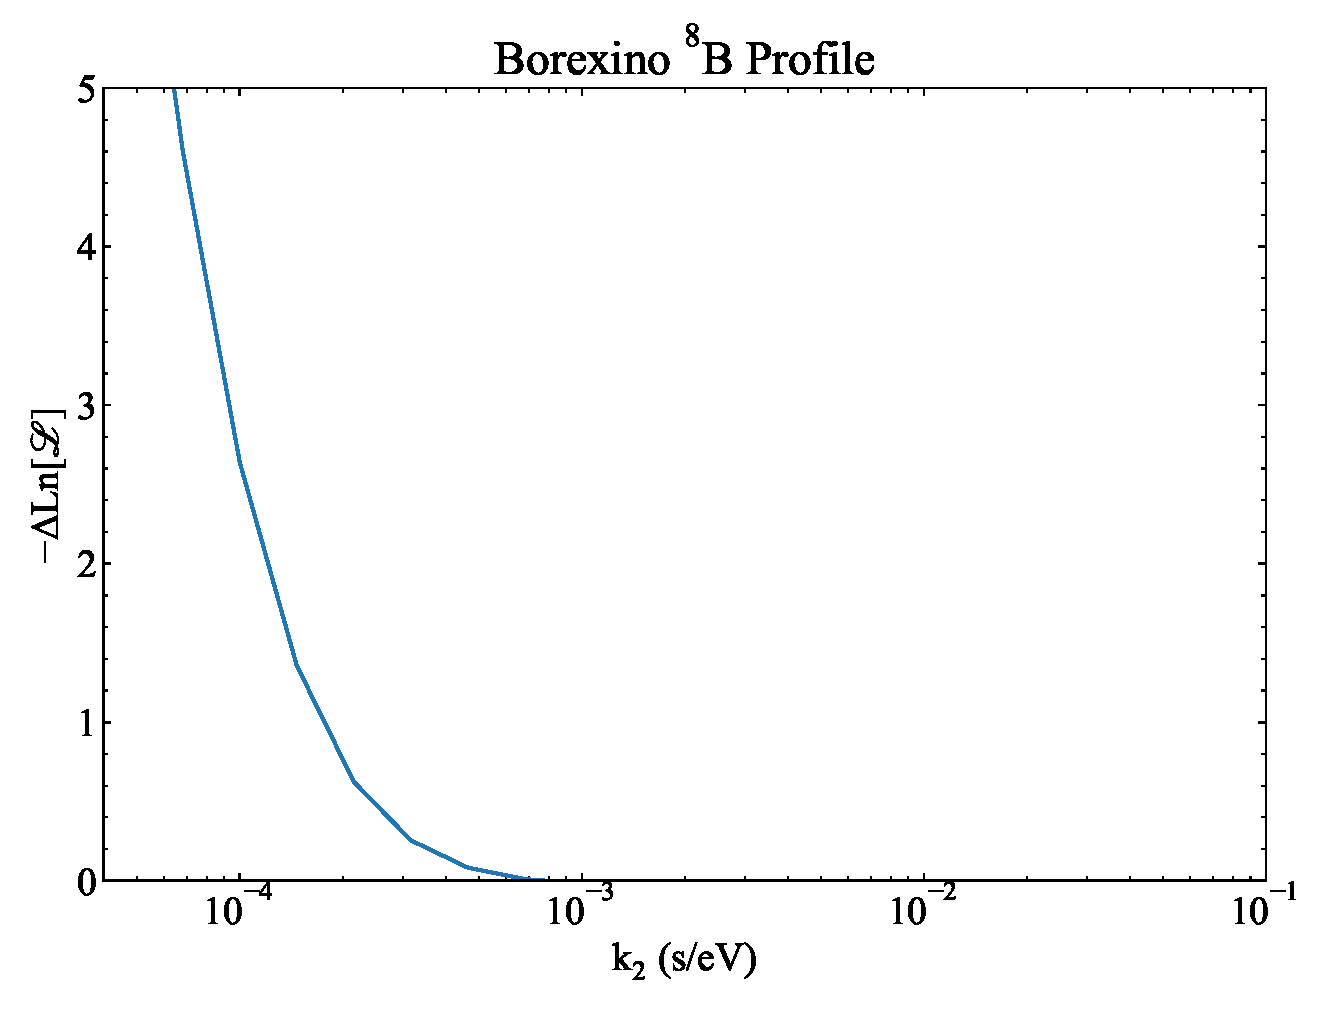
\includegraphics[width=0.58\columnwidth]{borexino_8b}
\includegraphics[width=0.58\columnwidth]{kamland_8b}
\caption{The profiled likelihood for the parameter $k_2$ using $^8$B measurements from SuperK~\cite{superkiv}, Borexino~\cite{borexino8b}, and KamLAND~\cite{kamland8b}.}
\label{fig:8b_profiles}
\end{figure}

\subsection{$^7$Be Constraints}

Borexino~\cite{borexino7be} and KamLAND~\cite{kamland7be} measured the 862 keV line of $^7$Be neutrinos which account for $90\%$ of the flux from this isotope. 
The average survival probability weighted by the $^7$Be production regions for 862 keV neutrinos is computed for any particular set of neutrino parameters.
Using these survival probabilities, the measured $\Phi_e$ of each experiment is converted to a true $^7$Be flux with \Cref{flux_conv} and compared to the SSM prediction with \Cref{combolike}. 
As these neutrinos are much lower energy, they contain a significant fraction of mass state one. 
Here the lifetime of mass state one, $k_1$, is treated as a nuisance parameter and floated in the fit. 
The profiles in \Cref{fig:7be_profiles} are generated by scanning $k_2$ while floating neutrino parameters and $k_1$.

Note that these constraints are stronger than $^8$B constraints because these neutrinos are lower energy, so measured fluxes near the SSM prediction - even with less precision - can rule out shorter lifetimes.
This holds true to some extent for radiochemical gallium and chlorine experiments discussed in following sections.

\begin{figure}
\centering
\includegraphics[width=0.58\columnwidth]{borexino_7be}
\includegraphics[width=0.58\columnwidth]{kamland_7be}
\caption{The profiled likelihood for the parameter $k_2$ using $^7$Be 862 keV line measurements from Borexino~\cite{borexino7be} and KamLAND~\cite{kamland7be}. Note the shape of the Borexino profile is quite similar to KamLAND, just excluding short lifetimes at higher significance due to being a more precise measurement results in going off the scale of these plots.}
\label{fig:7be_profiles}
\end{figure}

\subsection{Gallium Constraints}

The SAGE~\cite{sagecombo} experiment has conveniently combined all gallium solar neutrino measurements into a single value: a rate of solar neutrino interactions on an atom of gallium. 
This requires a bit more effort than the $^8$B and $^7$Be measurements as this rate combines every type of solar neutrino flux, and is related to the fluxes by the gallium neutrino capture cross section.
It is most convenient to compute the expected interaction rate for a particular set of neutrino flux values and mixing parameters and compare this to the measured total rate. 
This follows the analysis described in Section V in \cite{sagecombo} with the notable exception that the survival probability used here includes neutrino decay.

For each type (that is, originating isotope) of solar neutrino, the average gallium cross section weighted by the energy spectrum and survival probability is calculated for a particular set of neutrino parameters using the appropriate production regions in the Sun for that type.
The gallium cross section used here is the same modified form used in the SAGE analysis~\cite{sagecombo}.
The sum of these average cross sections multiplied by the flux of each type yields the total interaction rate expected on gallium.
This quantity can be directly compared to the measured rate with a likelihood term similar to \Cref{combolike}.

A profiled likelihood is arrived at in a similar way as described above: neutrino parameters, SSM fluxes, and lifetime of mass state one are floated while $k_2$ is scanned. 
Neutrino parameters and SSM fluxes are constrained with the same priors as elsewhere in this analysis.
The result is shown in \Cref{fig:ga_profiles}.

\begin{figure}
\centering
\includegraphics[width=0.58\columnwidth]{gallium_8b}
\caption{The profiled likelihood for the parameter $k_2$ using the combined measurement of all gallium experiments~\cite{sagecombo}.}
\label{fig:ga_profiles}
\end{figure}

\subsubsection{Validation}

As this is more complicated than a simple constraint, some additional verification is needed to ensure there are no issues with the code.
To that end I have reproduced the per-component interaction rate from Table IV of~\cite{sagecombo} in \Cref{tbl:gallium} using the mixing parameters and approximate form of the survival probability from that same reference.
As these values are nearly identical to those reported in the original publication, my calculation of cross sections and total rates appears correct.

Note that~\cite{sagecombo} uses an approximate form of the survival probability whereas for all other parts of this analysis I have numerically diagonalized the MSW Hamiltonian (see \Cref{lifetime_model}).
A notable difference between these two approaches is that the approximate forms assume a uniform solar density for each flux, while my numerical method accounts for the density profile in the regions where these neutrinos originate.
Using my numerical computation instead of the approximate form yields slightly different numbers (also shown in \Cref{tbl:gallium}). 
Both total rates are consistent with the Gallium measurements $66.1\pm3.1$ SNU~\cite{sagecombo} at one sigma, and the numerical method is used for other parts of this analysis.

With the calculation of the expected rate validated, the remaining step of including gallium results in this analysis is a comparison to the measured rate with a term like \Cref{combolike}.

\begin{table}
\centering
\begin{tabular}{c|r|r|r}
Component & SAGE Rate (SNU) & Approximate $P_{ee}$ (SNU) & Numerical $P_{ee}$ (SNU) \\ \hline
$pp$		& 39.35	&	39.34 	&	39.18	\\
$pep$		& 1.43 	&	1.43 	&	1.35 	\\ 
$^7$Be		& 18.73	&	18.74	& 	18.78	\\
$^{13}$N	& 0.89 	&	0.89	&	0.85	\\ 
$^{15}$O	& 1.23 	&	1.23	&	1.13	\\ 
$^{17}$F	& 0.03 	&	0.03	&	0.03	\\
$^8$B		& 4.64 	&	4.63	&	4.54	\\ 
$hep$		& 0.02 	&	0.02	&	0.02	\\ \hline
Total		& 66.31	&	66.32 	&	65.80	\\ \hline
\end{tabular}
\caption{\label{tbl:gallium}Shown here are the predicted interaction rates of each neutrino flux with Gallium computed with the code developed for this analysis using both the approximate survival probability forms in~\cite{sagecombo} and the numerical forms used elsewhere in this analysis. The values published by SAGE~\cite{sagecombo} are shown for reference.}
\end{table}

\subsection{Chlorine Constraints}

The analysis of radiochemical measurements of interactions on chlorine is very similar to that of the gallium experiments described above. 
So, a similar analysis as done for gallium was performed here, but using the measured rate from the Homestake~\cite{homestake} experiment, $2.56\pm0.23$ SNU on $^{37}$Cl, along with the chlorine cross sections used for that analysis.
The result of the profile are found in in \Cref{fig:cl_profiles}.

\begin{figure}
\centering
\includegraphics[width=0.58\columnwidth]{chlorine_8b}
\caption{The profiled likelihood for the parameter $k_2$ using the measurements from Homestake~\cite{homestake}.}
\label{fig:cl_profiles}
\end{figure}


\subsubsection{Validation}
The Homestake~\cite{homestake} experiment does not go into detail about expected rates from separate components.
Also, the references cited there tend to assume $P_{ee} = 1$ when calculating expected rates which is not a useful comparison to make with this analysis.
A more recent paper~\cite{bachall_lma} does a modern calculation of the expected interaction rates per flux component that is directly comparable to the model used here.

Using the fluxes and mixing parameters quoted in Table I of \cite{bachall_lma}, I have reproduced the interaction rates central values for Chlorine in \Cref{tbl:chlorine} and compared to the LMA solution from Table I of \cite{bachall_lma}.
The column showing the 'old' parameters are using the fluxes and mixing parameters from \cite{bachall_lma} while the column showing 'new' parameters uses the SSM and mixing parameters used elsewhere in this analysis.
In all cases there is pretty good agreement with the measured rate from Homestake and between models.

\begin{table}
\centering
\begin{tabular}{c|r|r|r}
Component & \cite{bachall_lma} Rate (SNU) & 'Old' Parameters (SNU) & 'New' parameters (SNU) \\ \hline
$pp$		& 0.0	&	0.00 & 0.00		\\
$pep$		& 0.1 	&	0.13 & 0.12		\\ 
$^7$Be		& 0.46	&	0.45 & 0.30		\\
$^{13}$N	& 0.05 	&	0.05 & 0.02		\\ 
$^{15}$O	& 0.16 	&	0.17 & 0.07		\\ 
$^8$B		& 1.8 	&	1.82 & 2.20		\\ 
$hep$		& 0.1 	&	0.07 & 0.01		\\ \hline
Total		& 2.6	&	2.69 & 2.75		\\ \hline
\end{tabular}
\caption{\label{tbl:chlorine}Shown here are the predicted interaction rates of each neutrino flux with Chlorine both from an independent calculation \cite{bachall_lma}, using this analysis' code with the 'old' mixing and flux parameters in that reference, and again with the flux and mixing parameters used elsewhere in this analysis.}
\end{table}

\subsection{Combined Result}
\label{sec:combobreaker}

The likelihood profiles of individual experiments are multiplied (negative log likelihoods added) together to arrive at a combined likelihood profile shown in \Cref{fig:combined_profile}. 
Explicitly this includes: $^8$B measurements from KamLAND, Borexino, SuperK (I,II,III,IV) and this analysis of SNO data, $^7$Be measurements from KamLAND and Borexino, and total rate measurements from all gallium experiments (SAGE+GNO+GALLEX) plus the Homestake results on chlorine. 
The $99\%$ C.L. lower bound for the lifetime of mass state two is $>10.41\times10^{-4}$ s/eV. 
This is better than the the previous analysis for a few reasons: KamLAND results were not previously included, and both Borexino and Super-K published updated analyses compared to the data used in the previous limit. 
Notably the presence of a relatively significant minimum in the new SNO results is not particularly beneficial here since it occurs near the location of the limit.

\subsection{Cross-Check with Previous Limit}

The analysis that set the best limit~\cite{picoreti} did not go into detail as to how their analysis was performed, or which SSM values were used as a reference.
This makes it difficult to precisely reproduce their results, however since they do list the experimental results used, I can repeat my analysis using those experimental results and see if I get a similar limit.

The experiments used in the previous best limit were: Homestake (Cl), Sage (Ga), GNO+GALLEX (Ga), Borexino's first $^7$Be publication, SNO's 3-phase analysis, and Super-K (I). 
Homestake and the gallium experiments have not been updated and are handled as described above.
Borexino and Super-K (I) are handled as described above but with the less-precise flux determinations of those two analyses. 
The SNO 3-phase results are handled in an analogous way to Super-K results using only the flux information.


In \Cref{fig:cross_check_profile} I have combined the profiles from these measurements and arrived at a limit of $>7.58\times10^{-4}$ s/eV at $99\%$ C.L., a bit better than \cite{picoreti}'s quoted $>7.2\times10^{-4}$ at $99\%$ C.L..
That this is quite close to the limit set by~\cite{picoreti} indicates that these two analyses are consistent even if the methods presumably differ.
Unfortunately with the brevity of the previous paper a more direct comparison does not seem possible.

\begin{figure}
\centering
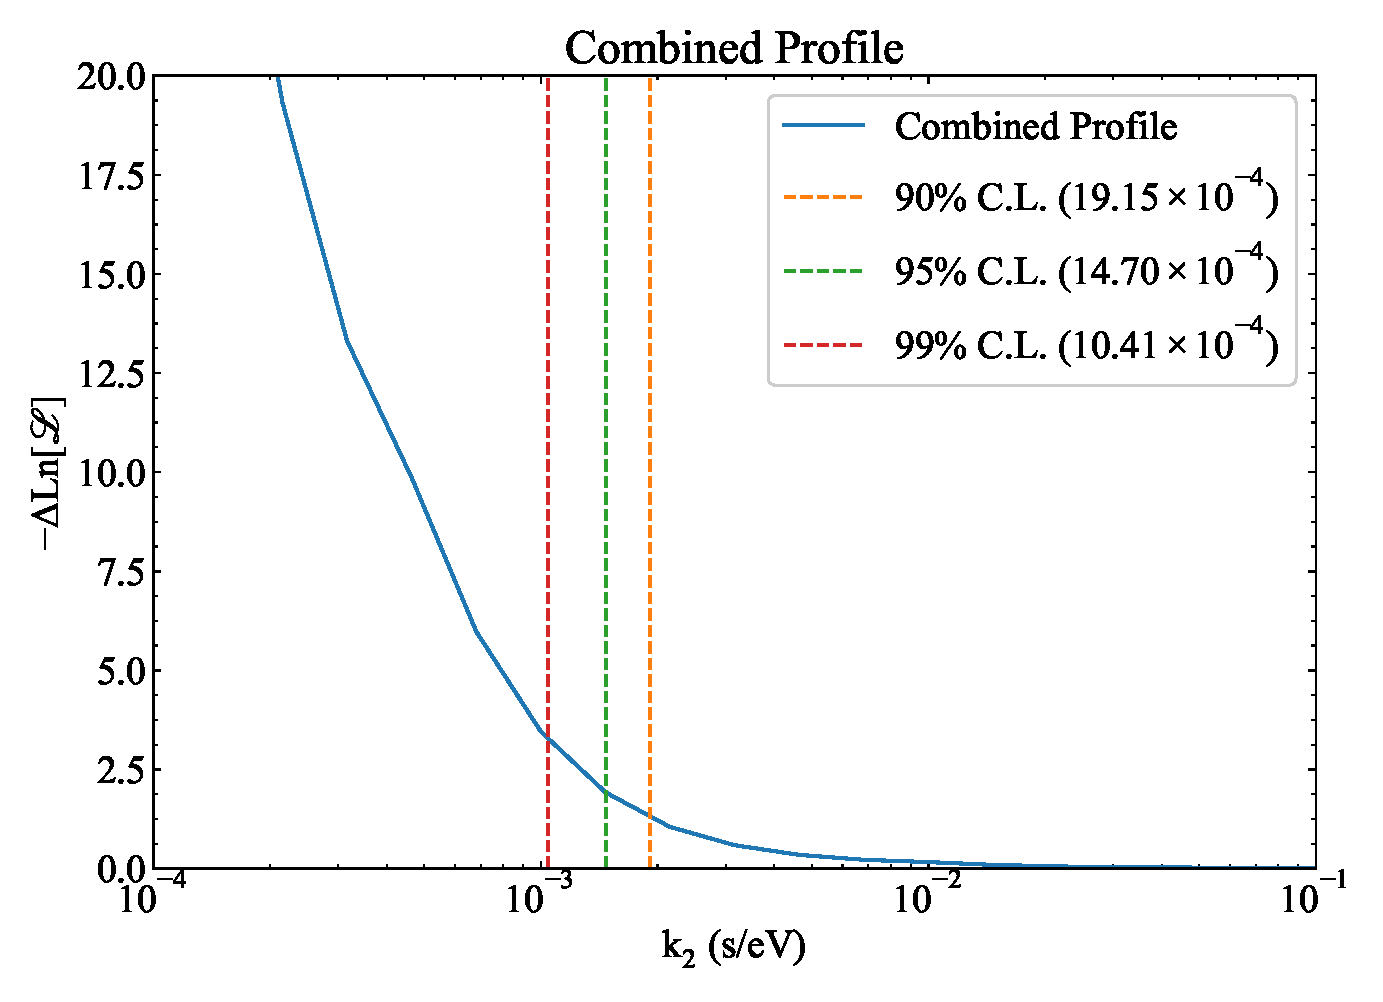
\includegraphics[width=0.95\columnwidth]{combined_profile}
\caption{The combined profiled likelihood described in \Cref{sec:combobreaker}.}
\label{fig:combined_profile}
\end{figure}

\begin{figure}
\centering
\includegraphics[width=0.95\columnwidth]{cross_check_profile}
\caption{The combined profile intended to reproduce the result in \cite{picoreti} by using the same experimental measurements. Notably the analysis methods are not identical so the results should be similar but do not match exactly.}
\label{fig:cross_check_profile}
\end{figure}
